\chapter{Implementation}

\section{Introduction}
Given the real-time nature of a CEP engine and the extensive uptime typical of a server, a thorough implementation is of maximum importance.

In this chapter I will explain how the project is structured and how it evolved in time, highlighting the choices made to find a balance between performance and convenience.

\section{Overview}
The T-Rex project, in its entirety, is composed of the engine library, a server, a client and an HTTP proxy. The engine, written in C++ and CUDA, is the foundation of the whole system and contains the business logic and the computationally intensive tasks. The server, written in C++ as well, links the core library and provides a network interface on top of it, receiving and dispatching packets for rules and events. The client, written in Java, allows full interaction with the CEP server via TCP/IP sockets: from publish-subscribe, to rule registration, using a TESLA parser created with ANTLR. The proxy, written in JavaScript for NodeJS, exposes an HTTP interface for publishing and subscribing, but at the moment doesn't implement rule parsing and registration. For the purpose of the thesis we will focus on the library, since its is the only one relevant in terms of feasibility and performance of static data integration.

At the beginning of the collaboration the T-Rex engine was a reasonably complex and well performing piece of software, although it showed several signs of its age. It was crafted over different iterations starting from 2010 and at that time C++ was still shaped according to its 12 years old original standardization. The very next year the C++11 standard came along, beginning an incredible period of renovation for both the language and the libraries, and the adoption of these new paradigms have the potential of a great improvement of safety and extensibility.\\
In particular the broad usage of dynamically allocated objects required exceptional caution during refactoring, because any minimal oversight could lead to leaks or attempts to access freed memory. In T-Rex it was handled with manual reference counting, which is now discouraged in favor of `shared_ptr`, that uses RAII to relieve the programmer from the responsibility of updating the count.\\
Similarly a big part of the execution relied on the combination of type unions, enums and switches to describe and process TESLA expressions. The access to the wrong type or the absence of a switch case can cause bugs that aren't detected by the compiler and lead to unexpected runtime failures. In the upcoming C++17 the type \emph{variant} will be added to the standard library and it uses the power of template metaprogramming to prevent those issues at compile time.\\
Moreover threading utilities and patterns are continuously evolving and they offer new levels of abstraction that reduce the needs of synchronization and locking, improving performances and preventing data races and deadlocks.\\
In addition to those safety benefits, there are several small improvements in terms of comprehensibility: like replacing array pointers with vectors, avoiding output arguments now that compilers handle efficiently the return statement, abandoning the cumbersome naming (inherited from the C tradition) for a wise usage of namespaces, adopting foreach loops and making use of idiomatic std functions.

These innovations highlighted the weak points of the original implementation and a renewal of the code base was deemed to be a collateral requirement of the broad modifications that the library was going to face. So, after an initial attempt of progressive refactoring, I proceeded with a complete rewrite of the engine in \emph{Rust}, a new language which offers the aforementioned advantages and even more.

\section{Rust}
Rust was born around 2010 as a side project of a Mozilla engineer and later backed by the company. The first pre-alpha release was reached in 2012 and the project hit version 1.0 in May 2015. So the language is pretty young and still missing some of its planned features, but many signs suggest that it may be on the right path.\\
First of all, while in the past there were several radical changes, after they reached the release 1.0 they committed to stability and backward compatibility, adopting a well defined workflow based on reference proposals. However the project has kept evolving quickly, with a release train model over 3 months windows.\\
Moreover it has raised a lot of interest within the community and there is a strong traction from a big company, ensuring continuity. Finally it is already used in production by Mozilla itself, Dropbox and Coursera among the others.

Rust aims to be a safe and practical language for system programming, with particular attention to concurrency. Its syntax, modern and expressive, combines the best aspects of imperative, object oriented and functional programming, offering the right level of abstraction for many different task.\\
The type-system, inspired by Haskell, is based on the concept of trait, which describe a property or a behavior of an object. Traits achieve their maximum utility in combination with generics, allowing code reuse while imposing clear restrictions on the applied types.\\
Rust also implements some features typical of higher level languages, like advanced union types (enums in Rust jargon), tuples, type inference, destructuring and pattern matching.\\
However the most prominent and peculiar characteristic is its unprecedented approach to safety with the concept of data ownership. Each object is tied to a single owner at a time, ownership can be transferred via assignment, return or function arguments and the content is moved and no longer accessible from the previous variable. If we want to access data without loosing ownership, it's possible to borrow multiple immutable references or a single mutable one, in the meantime the variable is considered blocked in something conceptually similar to a read-write lock. Every reference is bounded by the lifetime of the referee and can't outlive the owner. In this way is always clear who is responsible for the resource and when the owner goes out of scope the object can be safely dropped.\\
All these constraints and other minor ones are statically checked by the compiler, which gives strong guarantees of memory safety with no runtime overhead.

Last but not least it worth mentioning that there is a growing ecosystem of tools and utilities, that ease setup and development. For example: rustup.rs is an automated setup and update script, cargo is a modern and simple package manager, build tool and documentation generator, crates.io is the official repository of open source libraries, rustfmt is a customizable code beautifier and racer is a code completion utility. It's also thanks to this simplicity of bootstrap and distribution, that I was persuaded to adopt this new technology.

\section{Architecture}
The T-Rex rewrite, \emph{T-Rex2} from now on, is composed by three crates (Rust jargon for packages): `tesla`, that contains basic engine interfaces and language structures, `trex`, that is the implementation of those traits, and `benches`, a set of executables to test performances under simulated workload (on which we will focus in next chapter).

\subsection{Tesla}

\begin{figure}[h]
  \centering
  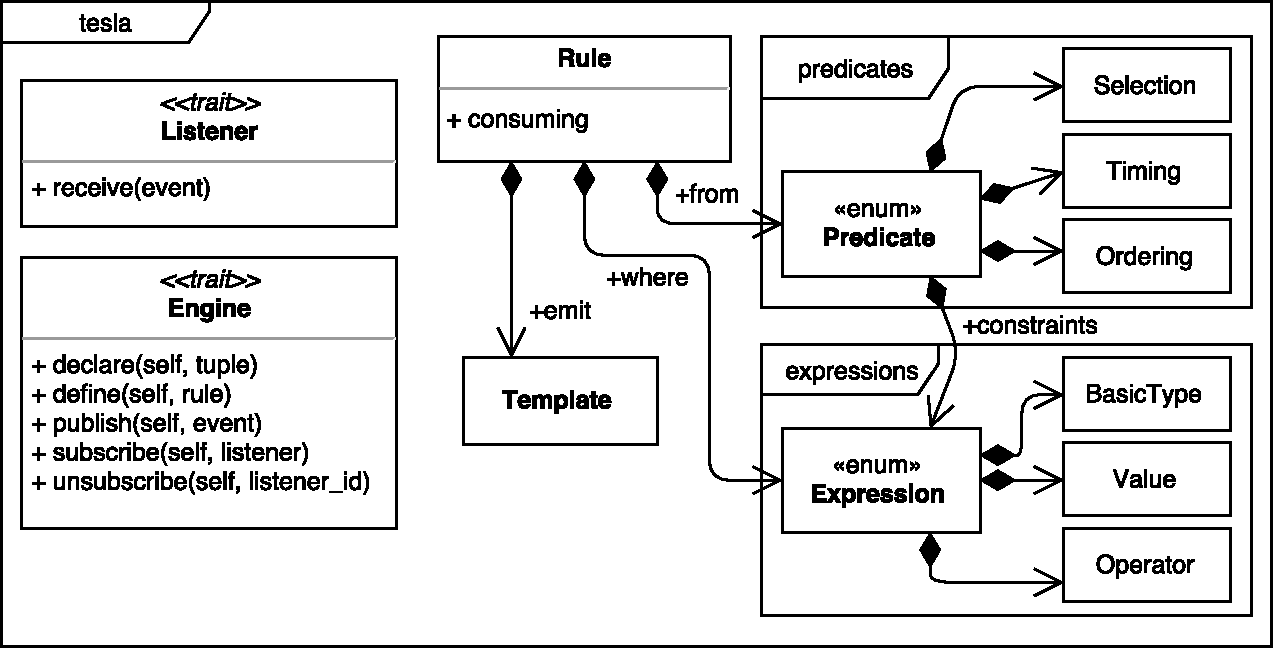
\includegraphics[width=\textwidth]{tesla_classes}
  \caption{Tesla crate overview}
\end{figure}

In tesla package I extracted all the aspects that aren't implementation related, so that it could work as minimal contact point between components like the library and the server. The core of the package is made of two traits: `Engine`, that defines methods for publish-subscribe, tuple declaration and rule definition, and `Subscriber`, that is used for event reception. Starting from these entry points the rest of the data structures just follows from the information required: in particular we have two sub-packages `predicates` and `expressions`, the first contains all the tools to describe patterns of events and static data, the latter contains the \emph{Abstract Sytax Tree} (AST) of algebraic and comparison expressions. They both heavily leverage rust native union type, giving them a terse design compared to the possible equivalent with C++ `variant`.

\subsection{TRex}

\begin{figure}[h]
  \centering
  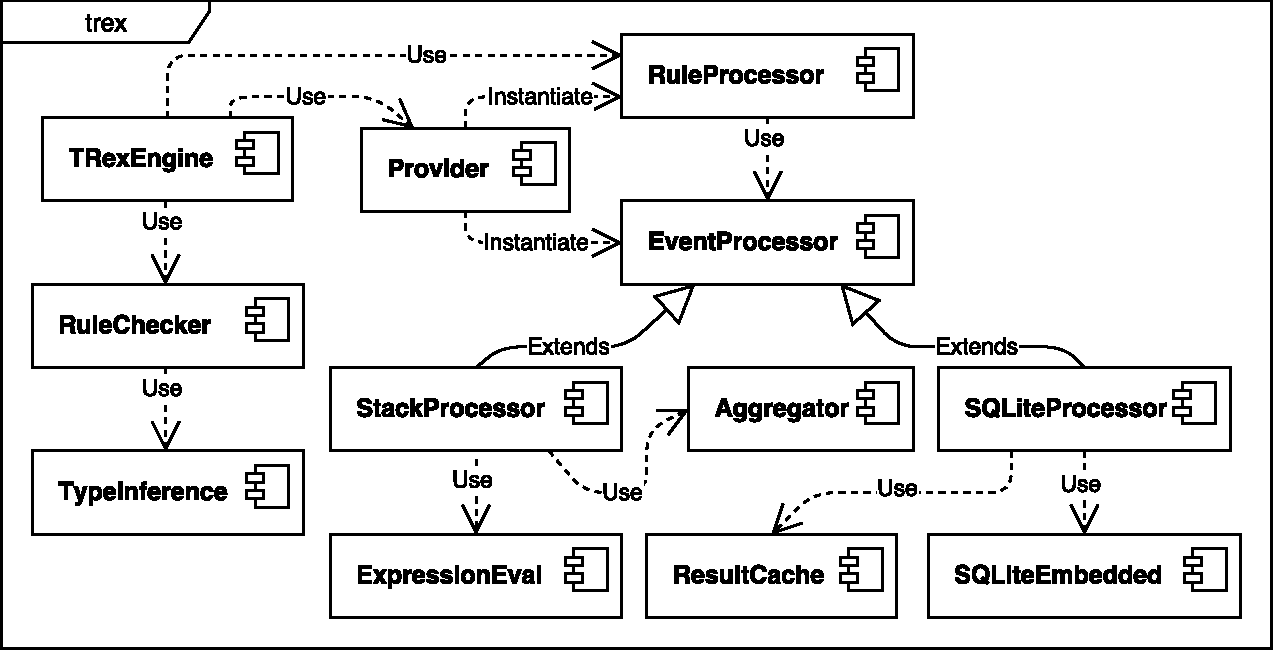
\includegraphics[width=\textwidth]{trex_components}
  \caption{TRex crate overview}
\end{figure}

The structure of `trex` crate closely recalls the previous implementation, with some simplification and new abstractions.

The core is the `TRex` struct, that implements the `Engine` trait and acts as a coordinator between the different components and the external world. The rest of the code can be divided in two main functionalities: the rule definition and the event processing.

The rule definition procedure is basically a sequence of configurations, that does not affect the performance of execution. When a new rule is received, `TRex` invokes the validation module and types, inferred from the collected tuple declarations, are checked to be used properly in expressions and assignments. If the rule passes the examination, a factory pattern is used to instantiate a dedicated `RuleProcessor`. Then the processor is indexed by the events that participate to the definition of the rule, so that is going to be activated only by those notifications that are relevant to its evaluation. In the original project the index was more sophisticated than a single hash-map and had a mechanism to filter the matches by checking those predicate constraints that only depend on immediate values. In practice the alternative appears to work well enough and additional optimization could be added if needed.

Event handling, instead, is the core of the business logic. Event notifications are sent to the `TRex` instance through the `publish` method, presented in pseudo-code in listing \ref{lst:publishmethod}. First the event is forwarded to the registered subscribers, then the index of rule processors is accessed and for each match a task is scheduled to execute in a thread pool, at this point the method is blocked waiting for tasks completion, finally if the evaluation does not produce new events the execution is complete otherwise the new events are submitted recursively to `publish` and the execution repeated. Since there is the assumption that incoming events are presented in time order and the blocking code prevent the next event from being processed, the time order for the generated complex events is guaranteed.\\
\begin{minipage}{\textwidth}
\begin{lstlisting}[caption={TRex publish method},label={lst:publishmethod},xleftmargin=.05\textwidth]
function publish(event):
  for_each subscriber in subscribers:
    subscriber.notify(event)
  done
  
  let processors = index.find_by(event.id)
  for_each processor in processors:
    thread_pool.execute { processor.process(event) }
  done
  
  let events = thread_pool.collect_results()
  for_each event in events:
  	self.publish(event)
  done
end
\end{lstlisting}
\end{minipage}\\
Going deeper, the `RuleProcessor`, which correspond to `StackRule` class in C++, is the coordinator of a sequence of `PredicatesProcessor` and its main method (in listing \ref{lst:processmethod}) is a generalized version of the Column-based Delayed Processing (CDP) algorithm that, as mentioned in chapter \ref{chap:tesla-trex}, is at the core of T-Rex library itself.\\
On event reception `RuleProcessor` is responsible of dispatching the notification to the predicates and, if the trigger is satisfied, of propagating the chain of evaluation. The evaluation is based on a list of objects called `PartialResult`, each them is a representation of sequence of tuples (events or static data) that are compatible with the pattern of predicates has been so far verified. Every step in the propagation consumes the list of partial results, filters it and enriches it with the predicate inner information, with the result that the list can be shrunk, expanded or dropped altogether. Once the evaluation is complete and successful, the `RuleProcessor` verifies the last constraints of the where clause and builds the events to emit from a template, possibly handling the consumption of some of the events used in the process.\\
\begin{minipage}{\textwidth}
\begin{lstlisting}[caption={RuleProcessor process method},label={lst:processmethod},xleftmargin=.05\textwidth]
function process(event) -> [event] :
  for_each predicate in predicates_processors:
    predicate.process(event)
  done

  results = []
  if trigger.is_satisfied(event):
    time = event.time;
    for_each predicate in predicates_processors:
      time = predicate.remove_old(time)
    done

    partial_results = []
    for_each predicate in predicates_processors:
      partial_results =
        predicate.evaluate(partial_results)
    done

    for_each partial_result in partial_results:
      if where_clause.is_satisfied(partial_result):
        results.push(template.fill_with(partial_result)
        mark_for_consumption(partial_result)
      fi
    done
  fi

  return results
end
\end{lstlisting}
\end{minipage}

In the previous version there were, clearly, only event based predicates and their different types (in term of event selection, aggregates and negations) were often coupled with business logic and in particular `StackRule` had to handle all of them explicitly, with specific functions and separate collections. T-Rex2 introduces a new abstraction, that is the aforementioned trait `PredicateProcessor` which is implemented by any component that acts as a predicate evaluator. In this way everything is handled uniformly: event and static processors are instantiated through a provider, for further decoupling, and kept into a unique list. Every time that a notification arrives all the elements of the list are notified and each of them decide how to handle the information. Similarly, during evaluation, the only mean of communication is through `PartialResult` and the nature of each step remains encapsulated.\\
This design choice makes it much easier to experiment with new data sources and hopefully this modularity will facilitate future development of custom components for different DBMS.

Currently the system runs two implementations of predicate processor: `EventProcessor`, which supports the previous functionalities and completes the CDP algorithm as in the original paper \cite{trex-cuda}, and `SQLiteProcessor`, that is the test implementation to interact with a relational database.\\
The `EventProcessor`, at every notification, filters the received event by ID and checking the constraint that depend only on immediate values, if everything matches the event is stored into a time ordered vector, which is periodically cleaned from old or consumed entries. When the evaluation starts and a `PartialResult` is received, the processor scans the events and propagates those that match every parameterized constraint.\\
The `SQLiteProcessor`, instead, doesn't interact with event notifications and it's activated only during the evaluation phase, when it queries the database to find suitable tuples, as we will see in the following section.

An example of rule processor is shown in figure \ref{fig:rule_processor}, where the rule is composed in sequence by a trigger, two event predicates and a static predicate. During the execution the two event processors have collected a stack of events, instead the SQLite processor has direct access to a DB table.

\begin{figure}[h]
  \centering
  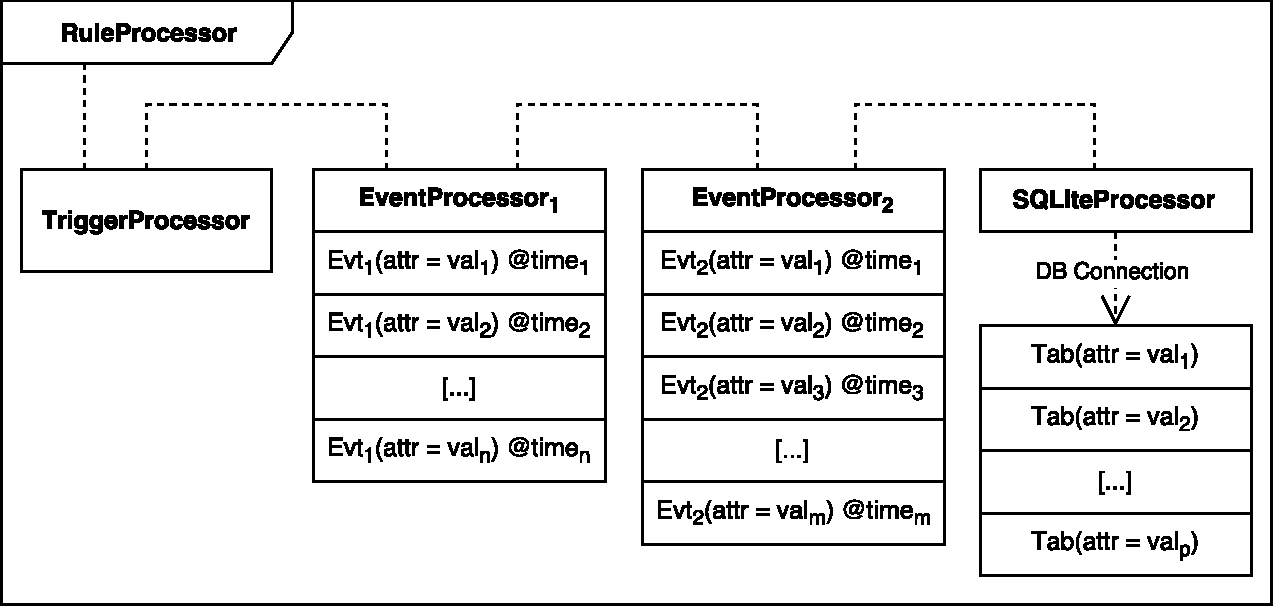
\includegraphics[width=\textwidth]{rule_processor}
  \caption{Processors chain example}
  \label{fig:rule_processor}
\end{figure}

\section{SQLite module}
The SQLite module contains two main components: a translator and an executor.

At creation time the predicate is fed to the translator and TESLA syntax is mapped permanently to a SQL statement using the following simple conversion rules.\\
The basic example is composed of an each predicate with no constraints nor parameters and, as we can see, the statement can be translated to a simple SQL select.
\begin{align*}% Example of each
&each\ SD\ \triangleq\\
&SELECT\ 1\ FROM\ SD;
\end{align*}
When the predicate features a negation, the operator `NOT EXIST` can be used to evaluate a subquery and return whether there are values in the result set or not.
\begin{align*}% Example of not
&not\ SD\ \triangleq\\
&SELECT\ NOT\ EXIST\ (SELECT\ 1\ FROM\ SD);
% For unexpected speed difference consider also:
% SELECT (SELECT id FROM SD) IS NULL;
% SELECT id FROM SD LIMIT 1;
\end{align*}
The selection policy $first$ does not have an implicit absolute ordering to work with, so it has to define one. The order clause is directly mapped to the SQL one.
\begin{align*}% Example of first
&first\ SD\ order\ by\ attr_1\ ASC,\ \ldots,\ attr_n\ DESC\ \triangleq\\
&SELECT\ id\ FROM\ SD\\
&ORDER\ BY\ attr_1\ ASC,\ \ldots,\ attr_n\ DESC\ LIMIT\ 1;
\end{align*}
For $last$ the same considerations made for $first$ hold, except for the mapping of the order clause, which is inverted.
\begin{align*}% Example of last
&last\ SD\ order\ by\ attr_1\ ASC,\ \ldots,\ attr_n\ DESC\ \triangleq\\
&SELECT\ id\ FROM\ SD\\
&ORDER\ BY\ attr_1\ DESC,\ \ldots,\ attr_n\ ASC\ LIMIT\ 1;
\end{align*}
The use of constraints inside tuple brackets find its correspondence in the SQL where clause.
\begin{align*}% Example of attribute constraint
&each\ SD(attr_1\ op \ val_1,\ \ldots,\ attr_n\ op \ val_n)\ \triangleq\\
&SELECT\ id\ FROM\ SD\\
&WHERE\ attr_1\ op\ val_1\ AND\ \ldots\ AND\ attr_n\ op\ val_n;
\end{align*}
The definition of a parameter it's processed adding its value to the query return column.
\begin{align*}% Example of parameter
&each\ SD[\$param = attr_i,\ \ldots]\ \triangleq\\
&SELECT\ attr_i\ as\ param,\ \ldots\ FROM\ SD;
\end{align*}
Finally the most common aggregation functions can be found in both the languages, so a translation is immediate.
\begin{align*}% Example of aggregates
&\$param\ =\ AGGR(SD.attr_1)\ \triangleq\\
&SELECT\ AGGR(attr_1)\ as\ param\ FROM\ SD
\end{align*}
The prepared statement produced is then stored for later use.

When the evaluation start, the executor populates the query with the parameters contained in `PartialResult` and execute it through `rusqulite` library (that is a wrapper of C SQLite embedded API) and the result are processed and forwarded in the chain of evaluation.

\section{Cache}
\label{sec:cache-impl}
To improve performance of data retrieval and try to keep the speed of execution above the constraints of real-time, a caching layer was added between the executor and the database.
\begin{figure}[h]
  \centering
  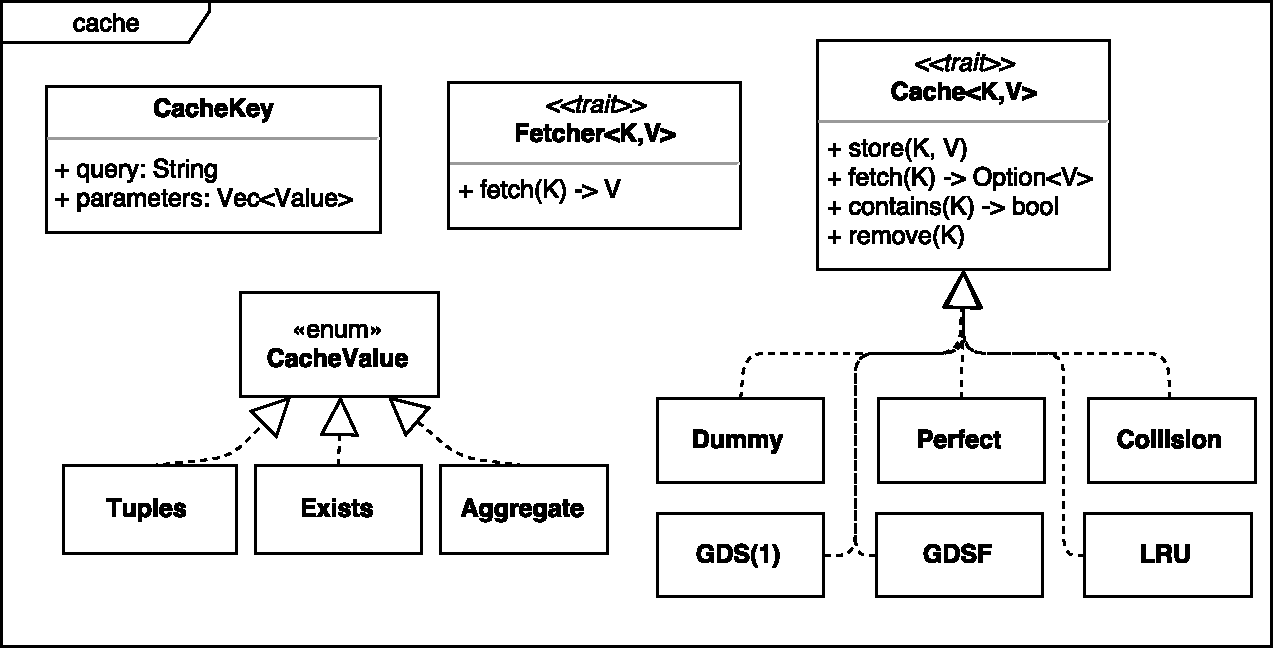
\includegraphics[width=\textwidth]{cache_classes}
  \caption{Cache module overview}
  \label{fig:cache_classes}
\end{figure}

The key of the cache is made by the combination of a SQL statement and the parameters with which it was populated. The key is intuitively unique for each result set\footnote{For the purpose of the thesis the data are considered immutable and cache invalidation is omitted} and it is also descriptive of the interrogation itself. So, instead of contacting the cache and database directly, the `SQLiteProcessor` will construct a key and delegate the task to a `Fetcher`. This new component will attempt a lookup in the cache and if the result is missing will fall back to the DB, hiding the complexity of cache update and multi-threaded synchronization.
The cache value is the result of a previously executed query and, depending from the type of the predicate, it can be a list of tuples or the result of an aggregate function or a flag of existence.

The system is integrated with several cache algorithms that can be activated and configured through the engine construction arguments.\\
Each of them, as can be seen in figure \ref{fig:cache_classes}, implements `Cache` trait allowing to easily replace one implementation with another.\\

\subsection{Simple Caches}
We can categorize the first three algorithm as simple caches, because they have basic storage approaches and do not leverage the context information to chose what to preserve and what to discard.
\paragraph{Dummy} The first implementation is a dummy cache that doesn't store anything and it's useful for testing the system in condition of 100\% misses. The methods `store` and `remove` are just empty, while `contains` will always return false and `fetch` will always `None`.
\paragraph{Perfect} The perfect cache is the opposite of the dummy and will store everything, without capacity limits. Its purpose is to test the maximum theoretical benefits of a cache. The methods simply forward the calls to those of an hashmap.
\paragraph{Collision} The collision cache is basically an hashmap with a reduced key space and a fixed capacity. The methods `contains`, `fetch` and `remove` act in the same way a normal map would. However the insertion possibly removes a single entry with the same hash value.\\

\subsection{Complex Caches}
The last three algorithms, instead, store metadata about the entries and exploit the context information to provide better chance to preserve useful entries in their limited available capacity.\\
\begin{minipage}{\textwidth}
\begin{lstlisting}[caption={Complex cache insertion},label={lst:complex-insertion},xleftmargin=.15\textwidth]
function store(key, entry):
  insert entry
  while memory usage > capacity
    remove the entry with least priority
  done
end
\end{lstlisting}
\end{minipage}\\
All the algorithms presented, as most of the caches in general, are characterized by an insertion method that operates, as shown in listing \ref{lst:complex-insertion}, by storing the new element to cache and removing the lowest priority element until the memory usage is below the allowed capacity. The difference between the three implementations is only the formula they use to compute priorities. All the other methods behave as in a standard map, except that `fetch` and `contains` function internally update the priority of the accessed element.

\paragraph{LRU-SIZE} \emph{Least Recently Used} is a family of caches that keep track of the order of access and prioritize time locality. In its usual implementation is meant for fixed size entries and, since in our case results sets can vary significantly in length we adopted the LRU-size variant. LRU-size has a maximum capacity set in terms of object sizes and, every time a value is inserted, multiple entries can be evicted to make room for the new one, keeping a controlled memory footprint. The cache was implemented on top of a `LinkedHashMap`, that is an hash map whose entries are connected one another in a linked list, having $O(1)$ complexity for each operation.

\paragraph{GDS(1)} \emph{Greedy-Dual Size(1)} \cite{gds1} is a cache developed in the context of web browsers and proxies. GDS(1) rewards small entries, so that in the same capacity will fit more values, increasing the probability of a hit. The priority is computed with the following formula:
\begin{align*}
priority\ :=\ 1\ /\ size\ +\ clock
\end{align*}
Where $clock$ is an aging factor to avoid stagnation of entries that aren't relevant anymore and it's updated monotonically as the priority value of the last discarded entry.

\paragraph{GDSF} \emph{Greedy-Dual Size Frequency} \cite{gdsf}, an evolution of GDS(1), is the current champion among the web caching algorithms and implemented, for example, by Squid caching proxy. It tries to consider a combination of how costly it is to obtain the entry, the size it occupies and the frequency it was accessed so far, with the following formula:
\begin{align*}
priority\ :=\ cost\ *\ frequency\ /\ size\ +\ clock
\end{align*}
Where $clock$ is the same aging factor seen for GDS(1).

Both GDS(1) and GDSF can be implemented using a expecially crafted combination of a binary heap and an hash map, with amortized $O(1)$ complexity and worst case of $O(log(N))$. However, for simplicity, it has been implemented using a high level combination of a B-tree set and an hash map, with complexity $O(log(N))$.
